\section{Methods}

\subsection{Data}

\subsubsection{Sources of data}

Human skin tissue was excised from cadavers and healthy subjects for previous studies at the Red Cross Hospital in Beverwijk, the Netherlands~\sidecite{Haasterecht2023, Zhou2023}.
Pieces of these tissues were imaged with multiphoton microscopy and their stress-strain response curves were measured mechanically, see \cref{fig:lab-setup}~\sidecite{Haasterecht2023, Zhou2023}.
Data is acquired in batches from April 2021 until July 2022.
Development and testing data come from the same source.

\begin{figure*}
    \centering
    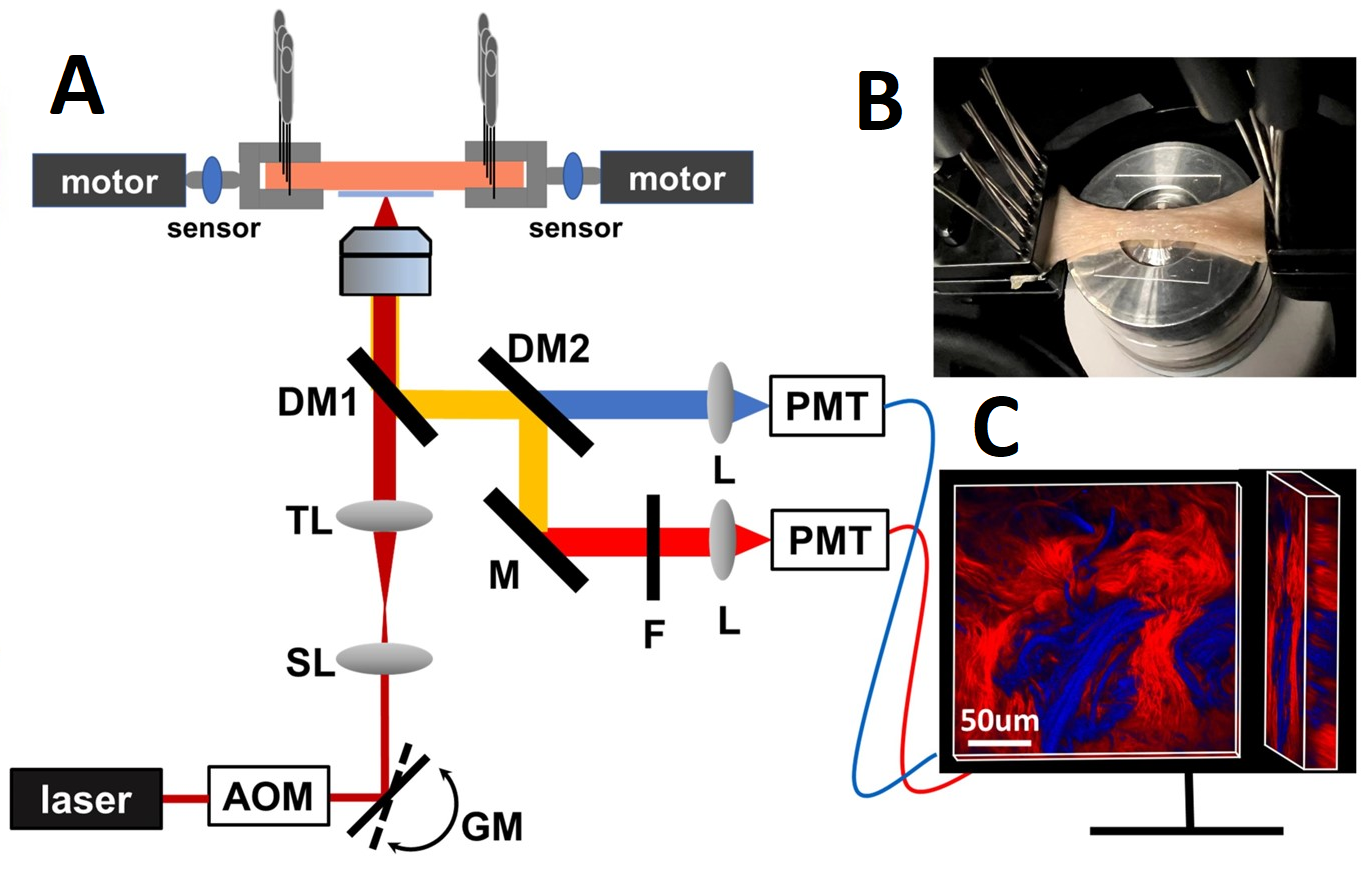
\includegraphics[width=\linewidth]{skinstression/images/measuring-setup.png}
    \caption[Skin stretch setup]{
        Skin stretch setup.
        The schematic of the experimental setup (A) shows a femtosecond pulse laser, which central wavelength is 1050 nm with pulse duration less than 80 fs; AOM- acousto-optic modulator; SL-scan lens; TL-tube lens, focus tunable; DMP1-dichroic mirror reflecting backscattering signals from fundamental photons; DMP2 dichroic mirror splitting 2PEF and SHG channels; M- Mirror; F- bandpass filter, F520/35; L- focusing lens; PMT-photomultiplier tube detectors. 
        The PMT signals are shown as image stacks (C) where red color represents collagen fibers and blue color represents elastin fibers.
        A photograph of the skin stretching for \qty{150}{\percent} is shown (B).
        Adapted with permission from \fullcite{Zhou2023} (Ref.~\cite{Zhou2023}).
    }
    \label{fig:lab-setup}
\end{figure*}

It is unknown if individuals received treatment relevant for this study.

The sample size is arrived at taking into account all previously included subjects and excluding abdomen data and scar tissue.
This amounts to a total of 1649 SHG images from 63 samples to train on.
% For a detailed summary of the number of samples, see fig. (graph with nodes and edges explaining number of images/curves).
Due to the limited amount of participants, individuals with unknown gender or age were included.

\subsubsection{Data preprocessing}\label{sec:skin_data_prep}

Depth stack images with a size of $1000\times 1000$ with a planar resolution of \qty{1}{\micro\meter} of all skin tissues were kindly provided by M.\ Zhou.
All stacks were separated into slices.

Images consist of three channels: third and second harmonic generation, and autofluorescence.
The SHG channel is chosen as it is assumed to only contain collagen information.

The SHG images are enhanced with contrast limited adaptive histogram equalization (CLAHE)~\sidecite{Zuiderveld1994ContrastLA} using scikit-image~\sidecite{scikit-image} to equalize importance of dark and bright regions.

The enhanced images are then transformed with a Yeo-Johnson transform using Scipy~\sidecite{2020SciPy-NMeth} such that the histogram of all images is as normal as possible.
Normalization generally accelerates training~\sidecite{Huang2020}.

The transformed images are standardized by subtracting the total mean and total standard deviation of the complete transformed image set, like
\begin{equation}
    X_\mathrm{out} = \frac{X_\mathrm{in} - \mu}{\sigma},
\end{equation}
where
\begin{equation}
    \mu = \frac{1}{N} \sum_i \sum_j \sum_k X_{i,j,k},
\end{equation}
and
\begin{equation}
    % \sigma = \sqrt{\frac{1}{N} \sum_{i,j,k} X_{i,j,k}^2 - \left(\frac{1}{N} \sum_{i,j,k} X_{i,j,k}\right)^2},
    \sigma = \sqrt{\frac{1}{N} \sum_i \sum_j \sum_k \left(X_{i,j,k} - \mu\right)^2},
\end{equation}
with $N$ the total number of pixels, $k$ an individual image and $i,j$ the pixel in the horizontal and vertical dimension, respectively.

The images are resized to $258\times258$ to fit into the neural network.

\subsubsection{Image selection}\label{subsec:image-selection}
SHG microscopy images from skin tissue suffer from optical phenomena.
The most evident problem is that imaging deeper into the tissue, photons are detected with less spatial accuracy because of scattering.
The deeper photons travel into tissue, the more possible paths photons can take to return to the detector.
Moreover, the chance of photons getting absorbed by the tissue increases with penetration depth.
Therefore, less photons get reflected from deeper tissue.

To counter these optical effects, inspired by \citeauthor{Koho2016} \sidecite{Koho2016} and \citeauthor{Blokker2022} \sidecite{Blokker2022}, measures to quantify image quality can be obtained.
With this, images can be sorted to this measure and the top $k$ images with best quality can be used to train the network, thus excluding noise.

Candidates for this measure are Shannon entropy, kurtosis, and skew for reasons explained in \ref{subsec:imq}
These quality measures are calculated per image using PyImageQualityRanking~\sidecite{Koho2016}, such that the quality measure can be validated by observing manually.

% \subsubsection{Image denoising}
% Another optical disadvantage of multiphoton microscopy is the occurrence of noise.\marginnote{Look up sources of noise.}

% Unfortunately, obtaining clearer images is hard.
% One way to reduce noise in the image is to use more photons.
% Either by averaging more images or increasing the amount of photons per image.
% Increasing the amount of photons penetrating the tissue increase the risk of damaging the tissue.

% Another way to deal with noisy images is to process the images.
% Promising denoising neural networks have been developed.
% The difficulty with this is that clean target data for supervised training is often not available in a biomedical setting.
% To counteract this, Noise2Noise (N2N) \cite{Lehtinen2018} was developed.
% Noise2Void N2V \cite{Krull2019}, a successor of N2N, does not rely on pairs of noisy images.
% Instead it only needs one image and corrupts it to use as target and learns a mapping between the noisy image and the newly created noisy image.
% This is useful if only one biomedical image is available.\marginnote{If denoising is used, move parts of this section to a theory section and refer to it here.}

% The original N2V model produces a checkerboard pattern.
% Noise2Void2 (N2V2) \cite{Hock2022} is an extension to N2V and reduces this artifact.\marginnote{Actually didn't do denoising, but if done, describe how here :)}

\subsubsection{Data augmentation}

To make the model more robust, data augmentation is applied.
Before resizing, the preprocessed images are cropped randomly from $1000\times1000$ to $700\times700$ preserving the aspect ratio.
The global brightness is adjusted randomly with $\pm \qty{30}{\percent}$.
The images are then randomly mirrored horizontally and vertically with a probability of \qty{50}{\percent}.
All data augmentations were performed with Torchvision \sidecite{torchvision2016}.


\subsection{Model}
The outcome of interest of the model are strain-stress response curves from SHG images from individual skin tissue pieces.
The model is named Skinstression (from skin stretch regression).
% The measurements were done mechanically by experimentalists.
% The measurement device itself is blind to clinical information.

This section shows the methods obtain a trained model from stress-strain curves and images to use it for inference and interrogate it with XAI techniques.
\Cref{fig:skin_stat_methods} shows the model development flow.

\begin{figure*}[p]
    \centering
    % 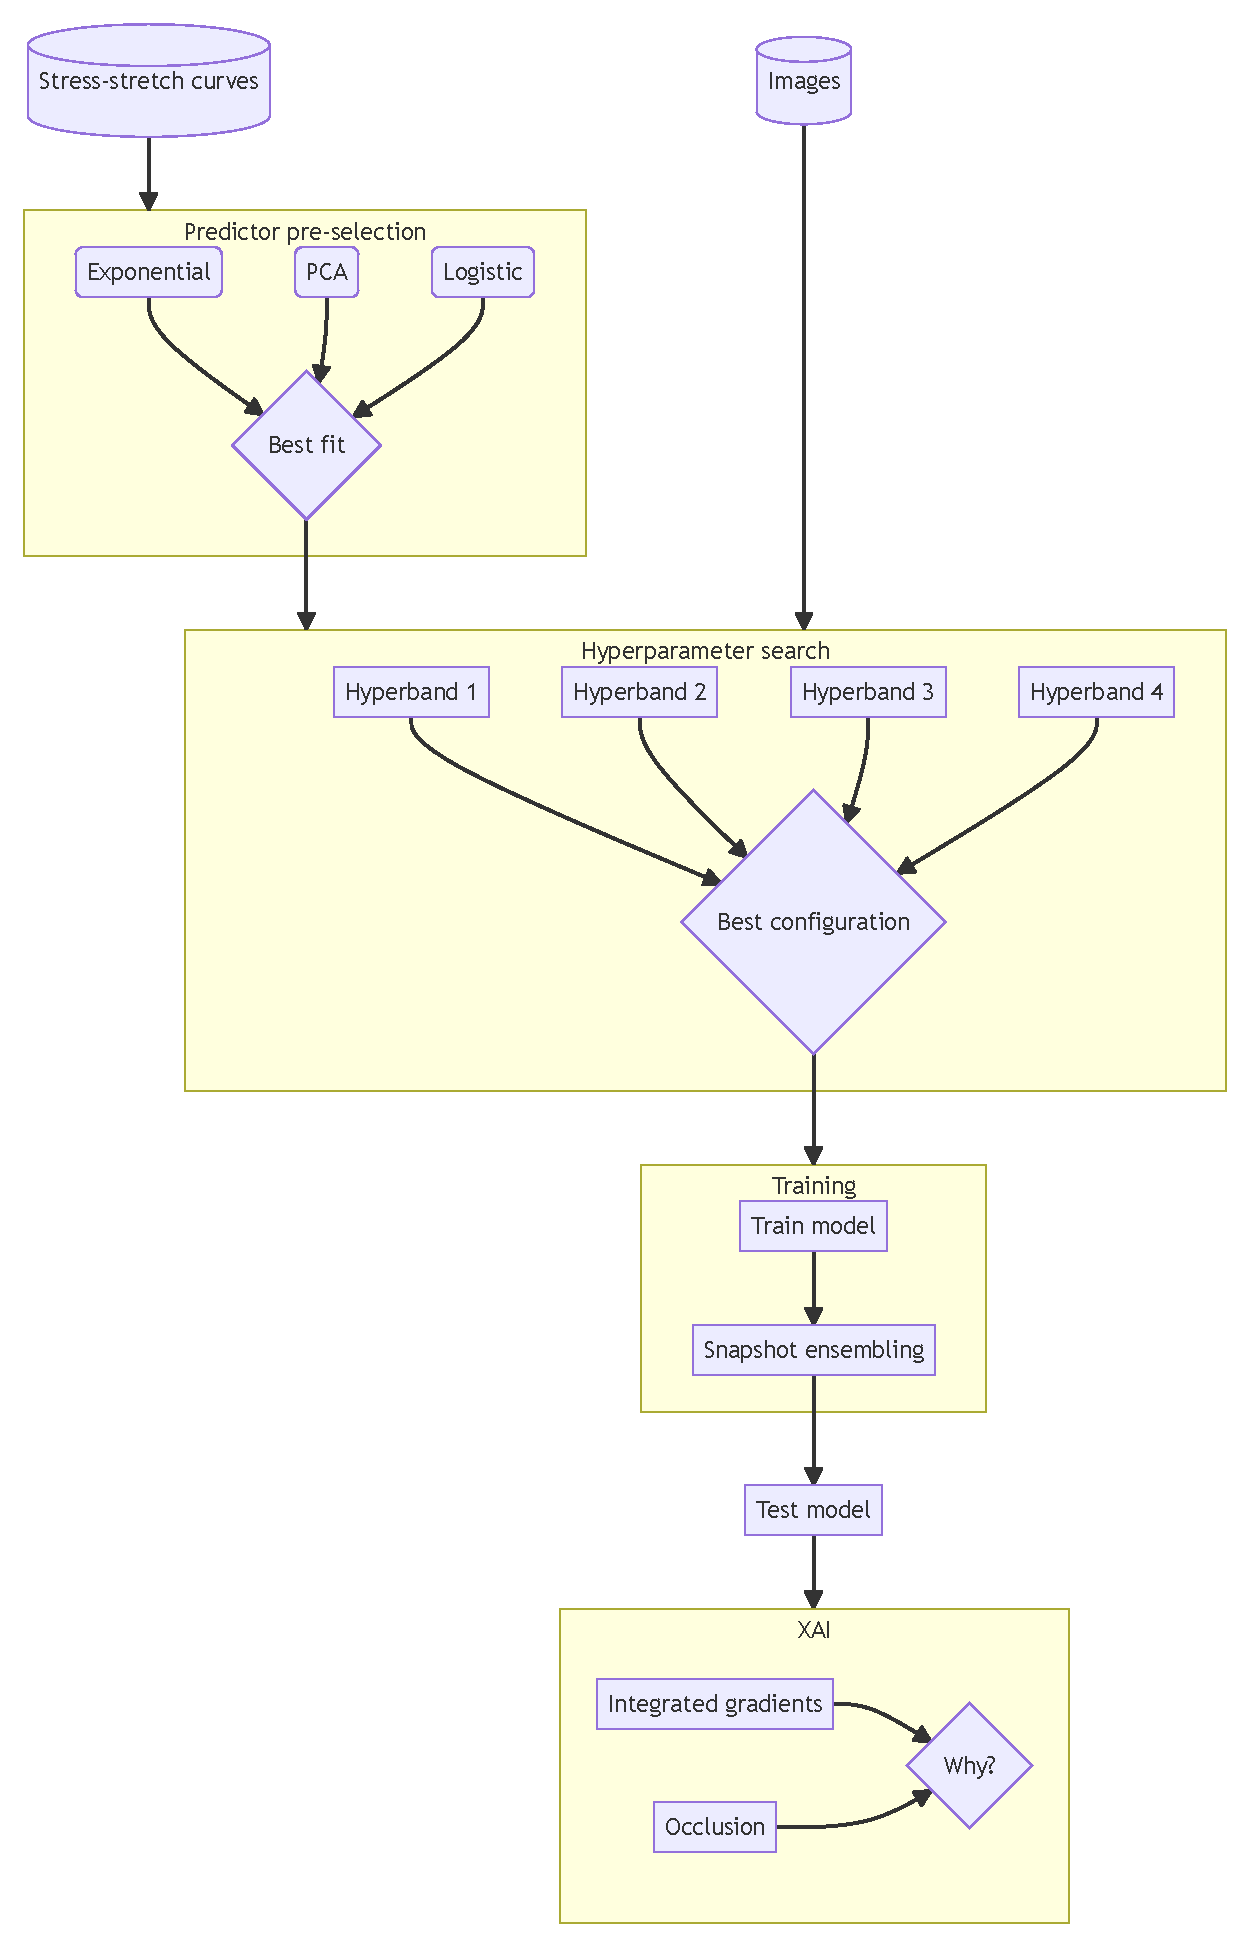
\includegraphics[height=\dimexpr\textheight-55.89pt\relax]{mermaid/skin_analysis.pdf}
    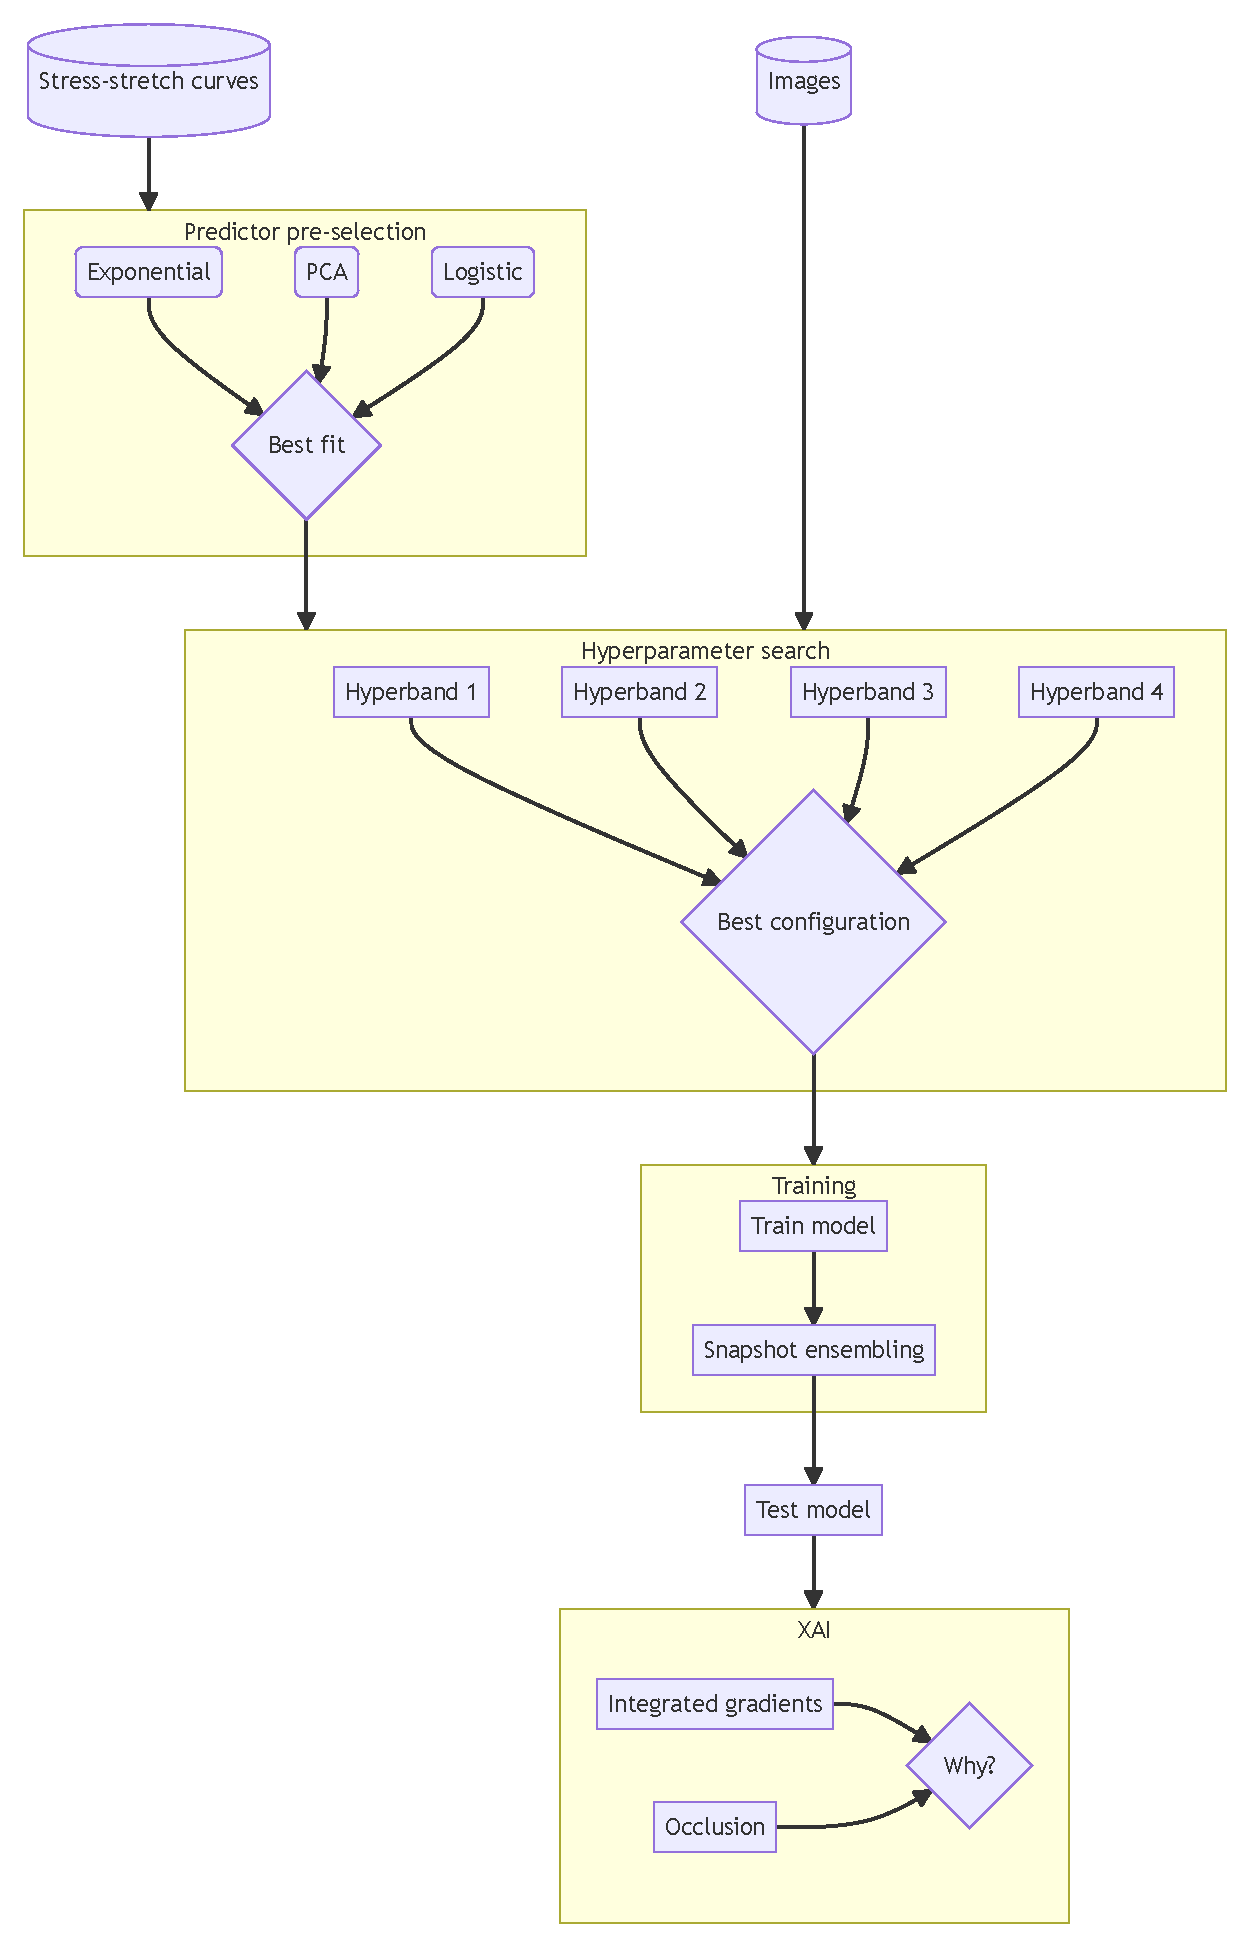
\includegraphics{mermaid/skin_analysis.pdf}
    \caption[Skinstression development flow]{
        Skinstression development flow.
        Exponentials, principal component analysis (PCA) reconstructions, and logistic curves were fit to the stress-strain curves.
        The best-fitted model was used to create training targets.
        The targets and images were used as input for further training.
        The hyperparameter search was performed by four Hyperband studies and the best configuration was used to train four models.
        The best validation loss determines the final model.
        The final model is tested and interrogated using occlusion and an adversarial attack.
    }
    \label{fig:skin_stat_methods}
\end{figure*}

\subsubsection{Predictor pre-selection}
As discussed in \cref{subsec:skin_predictors}, there are three predictor candidates.
These candidates are tested against the original strain-stress curves.

Strain-stress curves for all individuals were kindly provided by M.\ Zhou.
The curves only include points where the skin extension is larger than zero and the force positive.

\paragraph{Exponential and logistic curve}
The exponential and logistic models are fitted to all raw strain-stress curves with Scipy \sidecite{2020SciPy-NMeth}.
The optimal parameters were used as targets for training the model.
The goodness of fit is determined by the coefficient of determination (\cref{subsec:coef_det}).
A fit is considered good if $R^2 \approx 1$ and it passes reasonably through all data points.
In particular, the exponential regime of the fit should describe the leg part of the curve.

\paragraph{Principal component analysis}
PCA requires curves to align on at least one axis.
The first step to achieve this is excluding all stretch values above the stretch of the maximum of the shortest curve.
\citeauthor{Soylu2022} \sidecite{Soylu2022} did linear interpolation on the curves and restricted both stretch and stress to minim peak value.
PCA on two variables requires only one shared set of points.
Moreover, results of \citeauthor{Soylu2022} show knicks in the PCA reconstructions near the end of the curves, which could originate from a limited amount of data or linear interpolation.
Therefore, in this study, a non-uniform, univariate, interpolating spline was fitted to all points using Scipy~\sidecite{2020SciPy-NMeth} and the stress was calculated from the spline at the stetch values of the curve with the lowest maximum stretch.
After PCA on the complete dataset using Scikit-learn~\sidecite{Pedregosa2011}, the explained variance per component was calculated and used as a method to find an appropriate number of principal components.
From these principal components, the curves where reconstructed using \cref{eq:pca}.
The goodness of fit is determined by the coefficient of determination (\cref{subsec:coef_det}) and by eye.
A fit is considered good if it passes reasonably through all data points and has few inflection points.

Only if PCA on the full dataset works reasonably well, it is possible to use PCA on a subset and use it to reconstruct another subset.
This would be useful if PCA was used to construct predictors, as using PCA results of the full dataset introduce information leakage from the test sets to the training set, because the components describe data from both subsets.
This is unlike Ref.~\sidecite{Soylu2022} where information leakage was not considered.

\subsubsection{Convolutional neural network}
The basis of the model originates from Liang \emph{et al.} \sidecite{Liang2017} and is adapted by Soylu \sidecite{Soylu2022}.
The model, a convolutional neural network, consists of five blocks.
The first block consists of a convolutional layer with a $3\times3$ kernel, taking in one channel and have 64 channels as output.
The output is then normalized per batch using BN (\cref{sec:bn}).
The normalized batch is passed through a ReLU (\cref{subsec:relu}) layer.
After activation, three $2\times2$ maxpool (\cref{subsec:maxpool}) layers are applied.
The next second block is like the first block, but with a $5\times5$ convolution kernel and just one maxpool layer.
The third block is like the second block, but with a $3\times3$ convolution kernel.
The fourth block is like the second and third block, but with a $6\times6$ and without a maxpool layer.

The fifth block flattens the input and consists of a two linear layers.
The first linear layer maps 64 nodes to $N_\mathrm{nodes}$ nodes.
After the first linear layer, BN and ReLU activation is applied.
The second linear layer maps $N_\mathrm{nodes}$ nodes to 3 nodes.
A linear activation function ensures the output is continuous and unaltered.
The model is shown in \cref{fig:model}.

\begin{figure*}
    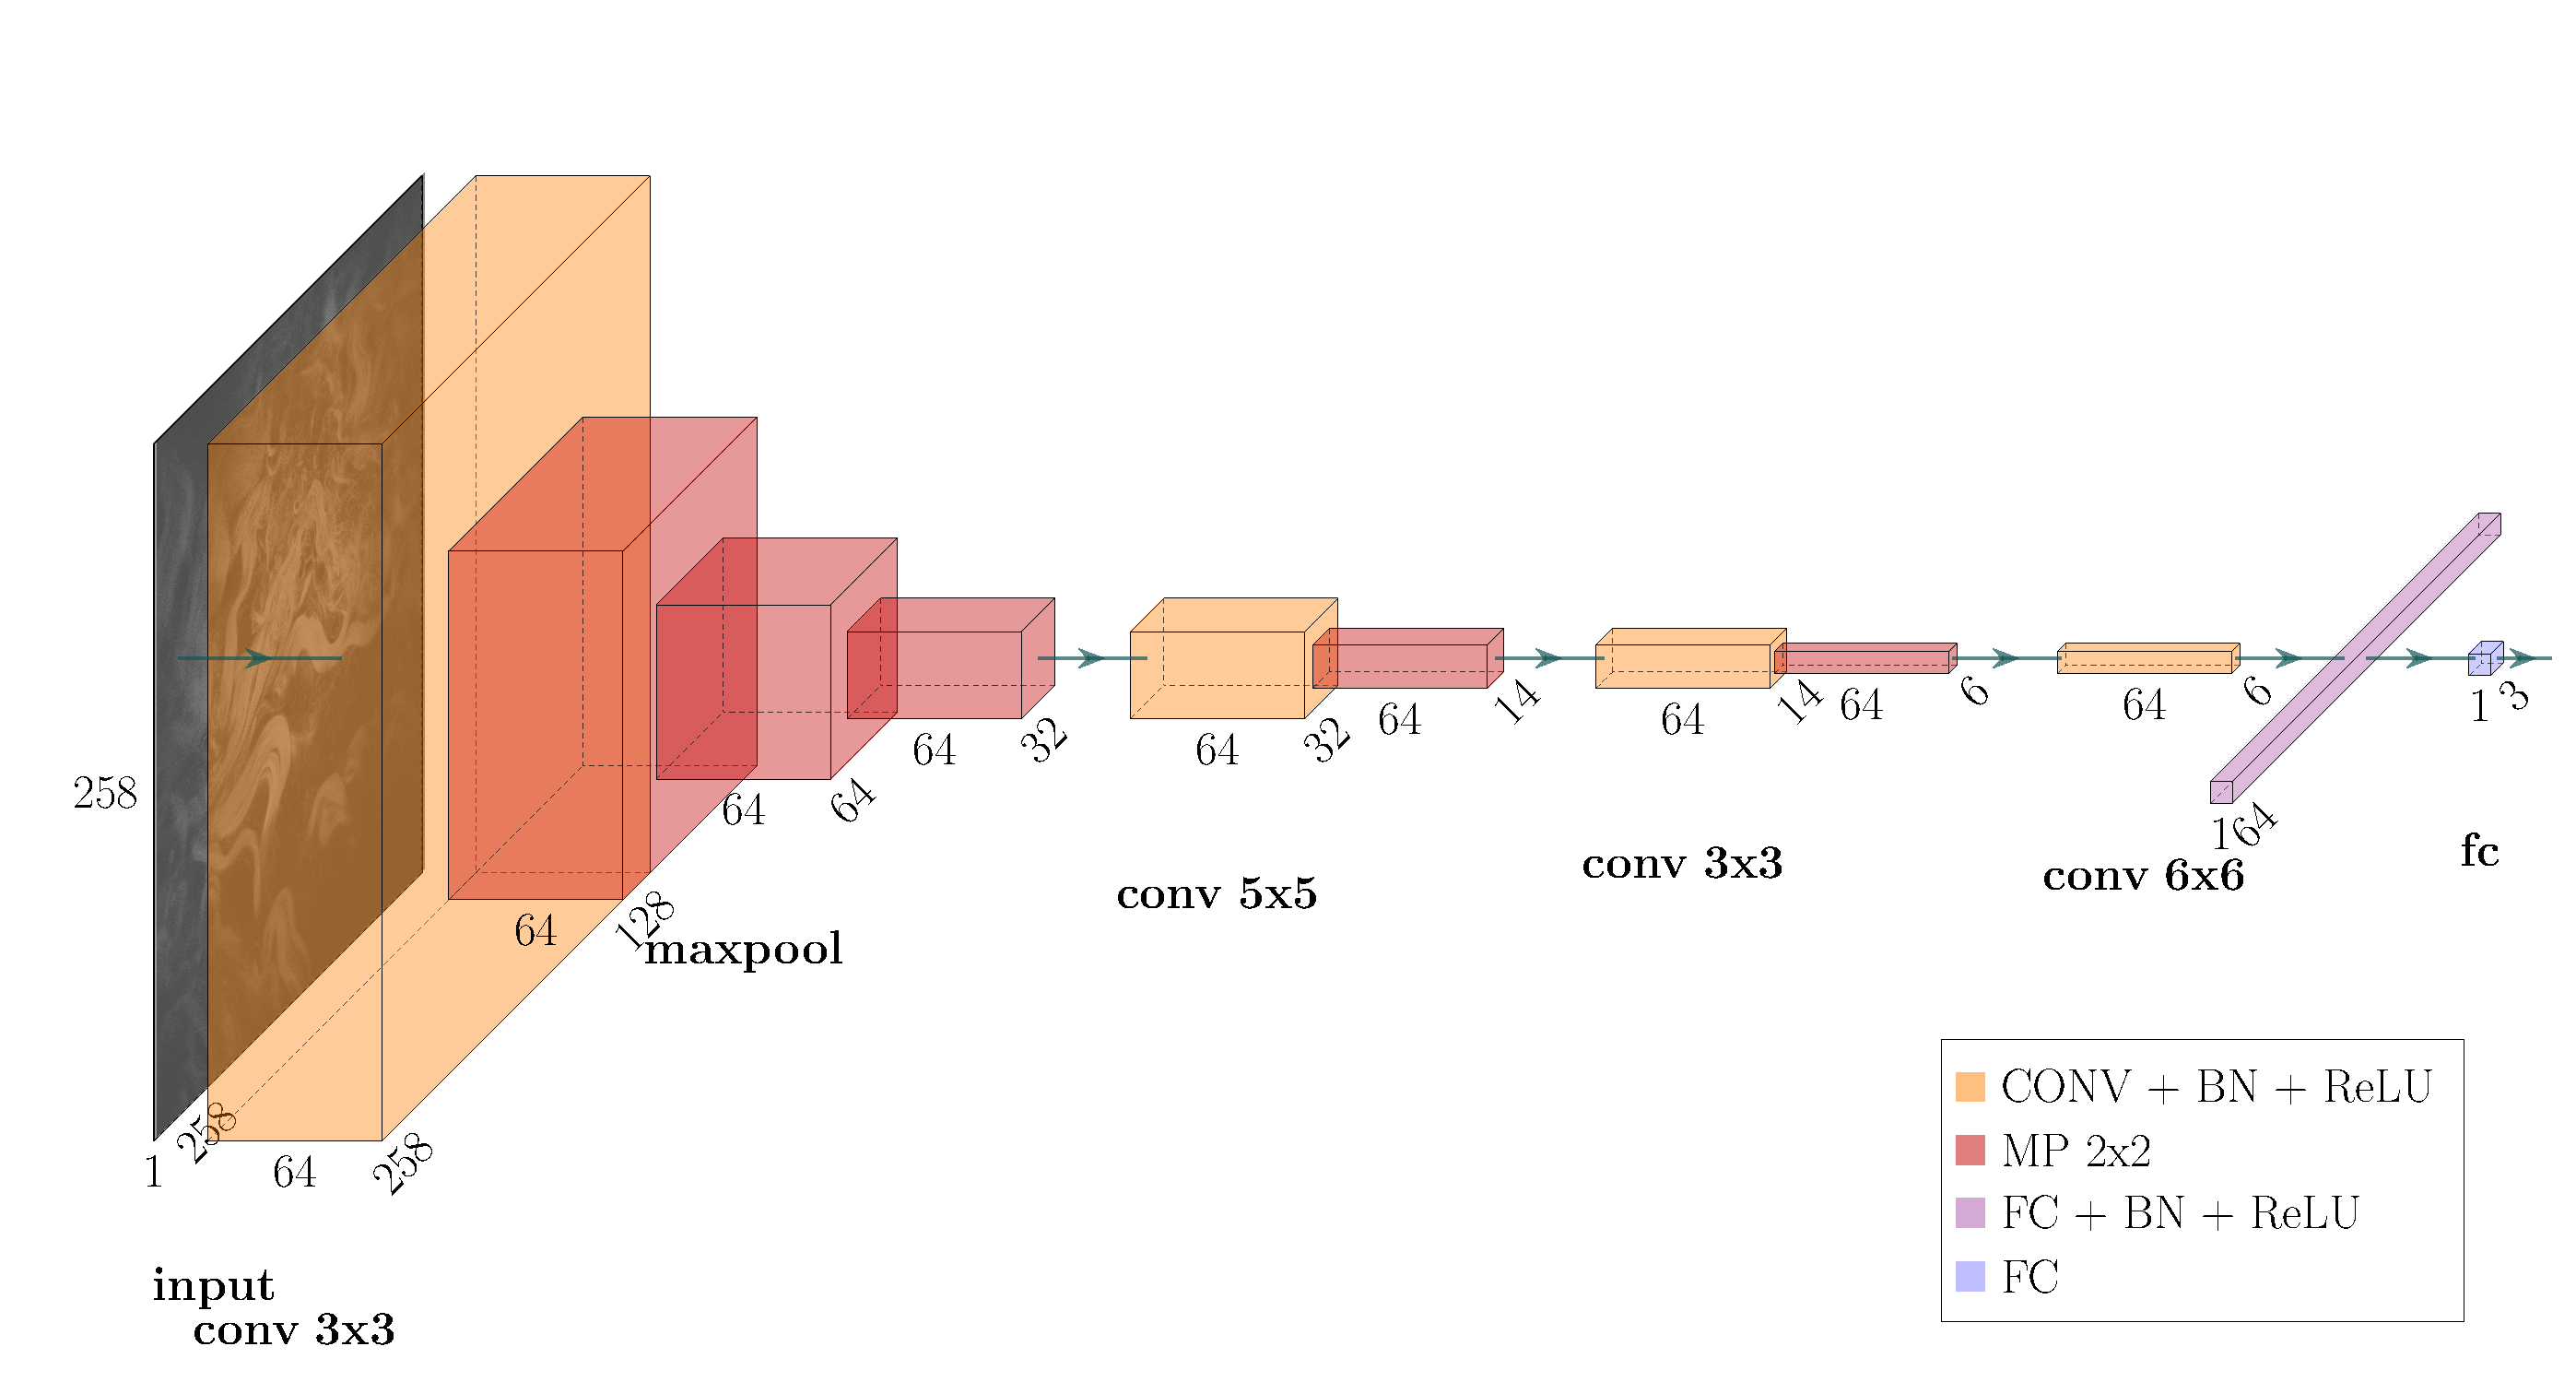
\includegraphics{skinstression/images/skinstression.pdf}
    \caption[Network architecture]{
        The convolutional neural network consists of five blocks.
        The first four blocks contain convolution, maxpooling, and batch normalization layers.
        The last block contains a fully connected network.
        It requires an input of $258\times258$ to get a vector of length 3 as output.
    }
    \label{fig:model}
\end{figure*}

The dropout layers in \sidecite{Soylu2022} are replaced by BN layers, as the input is not normalized and studies report better performance with BN.
Bias of all layers preceding BN layers have been set to zero to remove redundancy.

The neural network weights are initialized according to the method described by \citeauthor{He2015a} \sidecite{He2015a}, using a uniform transform.

\subsubsection{Hyperparameter optimization}
First, benchmark search 1 was done using Successive Halving with 100 trials.
See \cref{app:skin_conf_search_spaces} for a summary of configuration search space $\mathcal{C}$.
To allow trials to warm up, a minimum of 100 epochs were allowed.
To limit the trial duration, a maximum of 3000 epochs were allowed.
The number of trials were reduced with a reduction factor of $\eta=4$.
Trial parameters were sampled using the non-multivariate TPE algorithm.

The optimization was performed with the Adam optimizer ($\beta_1=0.9$, $\beta_2=0.999$), weighted focal MSE loss, and a cosine annealing with warm restarts learning rate scheduler.
Every trial used the complete dataset after data preparation (\cref{sec:skin_data_prep}).

The search uses a few data augmentations that are assumed to not alter the physical context of the image.
That is, force is exerted on the tissue unilaterally, which is horizontal in the image.
Therefore, flipping the image either vertically or horizontally is assumed to not change the stretch behavior.
Both flipping operations occur with a probability of $0.5$.
Moreover, the images' intensity is randomly changed uniformly by \qtyrange{0.7}{1.3}{\percent}.

To possibly find a more optimal set of hyperparameters, two searches with the Hyperband algorithm with 300 trials was performed.
Trial parameters were sampled using the multivariate TPE algorithm.
The learning rate was warmed up linearly for the first 20 epochs.

% As shown in [ref results search 1], it seems that the network has difficulty with estimating $\gamma_c$, while $E_\mathrm{max}$ and $\sigma_\mathrm{max}$ seem to be easier estimated.
% As the original stress-strain curves do not have data in the plateau regime, $\sigma_\mathrm{max}$ was given less importance in search 2 and 3.
% This was achieved by weighting individual targets of the focal loss, such that
% \begin{equation}
%     FL = \frac{FL_{\sigma_\mathrm{max}} + FL_{E_\mathrm{max} + FL_{\gamma_c}}}{3}
% \end{equation}
% Therefore, in search 2 and 3, the goal was to give less importance to $$

Search 2 introduces random $700\times700$ cropping to further artificially increase the number of available images to train on.
% Also included is the ability to weight the loss per target variable (not to be confused with LDS), to penalize hard variables more than easy variables.
% The targets were weighted as $(\sigma_\mathrm{max},E_\mathrm{max},\gamma_c) = (0.8, 1, 1)$, to give less attention to the plateau.
Search 3 includes the Yeo-Johnson transformation to see how input normalization affects the training outcome.

For a summary of the hyperparameter searches, see \cref{tab:skin_studies}.

Algorithms provided by Optuna \sidecite{Akiba2019} were used to choose trial configurations and keep track of trials.

\begin{table}
    \caption[Skinstression hyperparameter search studies]{
        Summary of settings for hyperparameter searches performed.
        Hyperparameters are grouped by operation type (image preprocessing, image augmenting, target weighting) and in applied order.
        Every search is done with the search space described in \cref{tab:conf_skin}.
    }
    \label{tab:skin_studies}
    \begin{tabular}{lcccc}
        % \toprule
        % Search                         & 1      & 2      & 3      & 4      \\
        % \midrule
        % CLAHE                          & \cmark & \cmark & \cmark & \cmark \\
        % Yeo-Johnson transform          & \xmark & \xmark & \cmark & \xmark \\
        % \midrule
        % Random $700\times700$ cropping & \xmark & \cmark & \cmark & \cmark \\
        % Intensity jitter               & \cmark & \cmark & \cmark & \cmark \\
        % Random horizontal flip         & \cmark & \cmark & \cmark & \cmark \\
        % Random vertical flip           & \cmark & \cmark & \cmark & \cmark \\
        % Random sharpness               & \xmark & \xmark & \xmark & \cmark \\
        % Random gaussian blur           & \xmark & \xmark & \xmark & \cmark \\
        % Random rotation                & \xmark & \xmark & \xmark & \cmark \\
        % \midrule
        % Target variable weighting      & \xmark & \cmark & \cmark & \cmark \\
        % \bottomrule

        \toprule
        Search                         & 1      & 2      & 3      \\
        \midrule
        CLAHE                          & \cmark & \cmark & \cmark \\
        Yeo-Johnson transform          & \xmark & \xmark & \cmark \\
        \midrule
        Random $700\times700$ cropping & \xmark & \cmark & \cmark \\
        Intensity jitter               & \cmark & \cmark & \cmark \\
        Random horizontal flip         & \cmark & \cmark & \cmark \\
        Random vertical flip           & \cmark & \cmark & \cmark \\
        Random sharpness               & \xmark & \xmark & \xmark \\
        Random gaussian blur           & \xmark & \xmark & \xmark \\
        Random rotation                & \xmark & \xmark & \xmark \\
        % \midrule
        % Target variable weighting      & \xmark & \cmark & \cmark \\
        \midrule
        Search algorithm               & SH     & HB     & HB     \\
        Multivariate TPE               & \xmark & \cmark & \cmark \\
        trials                         & 100    & 300    & 300    \\
        learning rate warmup           & \xmark & \cmark & \cmark \\
        \bottomrule
    \end{tabular}
\end{table}

\subsubsection{Training}
The AI was trained on a with LDS smoothed target variable distribution.
The targets were weighted with the inverse square root, to limit the impact of LDS.
Using the best configuration from hyperparameter optimization, a model is trained further for a total of 10000 epochs.
The learning rate scheduler was cosine annealing with warm restarts to allow for model ensembling later during inference\sidecite{Huang2017}, if deemed useful.
The learning rate was warmed up linearly for the first 20 epochs.
To see the influence of image quality, the model is trained using an ordered set of images.
The images are ordered with maximum entropy first and the model is trained on all images and the top 10, 20 and 30 images of every stack.
Moreover, to see the effect of using the original zoom level with the greatest detail at hand, the best 20 images of every stack were center-cropped to $500\times500$ and further randomly cropped to $258\times258$.
The lowest validation focal loss is used to compare model performance.
The model with the lowest validation loss is used for testing.

Pytorch~\sidecite{Paszke2019} was used to perform automatic differentiation on NVIDIA GeForce RTX 2070 Super GPUs on the BAZIS high performance computing cluster.

\subsubsection{Internal validation}\label{subsec:skin_dataset}
The thigh dataset is randomly distributed into a training (\qty{64}{\percent}), validation (\qty{16}{\percent}), and test (\qty{20}{\percent}).
The distribution is stratified by person, meaning samples corresponding to the same person cannot live in two subsets simultaneously.
The AI learns from the training set.
Every iteration, it is validated against the validation set.
During inference, the AI is applied to the test set as external validation.
The prediction is assessed by comparing it with measured strain-stress curves where $R^2$ is calculated with a \qty{95}{\percent} confidence interval.

\subsubsection{Bias study}
It is important to perform a study on bias for possible explanations of varying AI performance.
The samples were taken from individuals with varying age and gender.
Moreover, from some individuals, more mechanical measurements were taken.
Therefore, the age, gender, and number of samples were summarized.

% \subsubsection{Model selection}
% MISSCHIEN MODEL ENSEMBLING EN VALIDATION SET GEBRUIKEN VOOR VINDEN VAN BESTE AANTAL MODELS?
% The last $N$\marginnote{How many again?} models are ensembled together

\subsection{Explainability}

\subsubsection{Occlusion}
To explain the model output, occlusion \cref{subsec:occlusion} is used.
Using the Captum Python library~\sidecite{Kokhlikyan2020}, occlusion is done with $3\times3$ square patches moving with strides of 1.
All values in the patch have been replaced with 0.

\subsubsection{Adversarial attack}
To see the importance of homogeneous tissue within the skin tissue, black patches have been filled using Fiji \sidecite{Schindelin2012}.
Filling is done by drawing full white ellipses on top of the original image.
Moreover, in another attack, a black patch is copied to other locations in the image.
